\begin{definition}
$(X, M) $ - \textit{измеримое пространство}, где $X$ --- единица, $M$ --- $\sigma$-алгебра. Элементы $M$ называются \textit{измеримыми множествами}
\end{definition} 

$(\Omega, \F, P)$ --- вероятностное пространство

$(E, \Sigma)$ --- измеримое пространство

\begin{definition}
\textit{Случайный элемент} $X: \Omega \to E$, причём, $(\F|\Sigma)$ --- измеримое.
\end{definition}

\begin{definition}
$X$ --- $(\F|\Sigma)$-измеримое $\Leftrightarrow \ [\forall B \in \Sigma : X^{-1}(B) \in \F]$

$P_X(B) := P(X \in B) := P(\{w : X(w) \in B\})$
\end{definition}

$P_X(B)$ --- вероятность на $(E, \Sigma)$

\begin{definition}
$P_X(B)$ называется \textit{распределением вероятностей $X$}\\

В частности,

\begin{itemize}
    \item если $E = \R, \Sigma = B(\R)$, то $X$ --- \textit{случайная величина},
    \item если $E = \R^n, \Sigma = B(\R^n)$, то $X$ --- \textit{случайный вектор}
\end{itemize}
\end{definition}

\begin{theorem}[Критерий измеримости]
Если $\mathcal{M} \subset \Sigma, \sigma(\mathcal{M}) = \Sigma$, то $X$ --- $(\F|\Sigma)$-измеримо $\Leftrightarrow \forall B \in \mathcal{M} : X^{-1}(B) \in \F$
\end{theorem}

(Доказательство критерия известно из октч --- его могут спросить на доп вопрос, в билете это б/д).

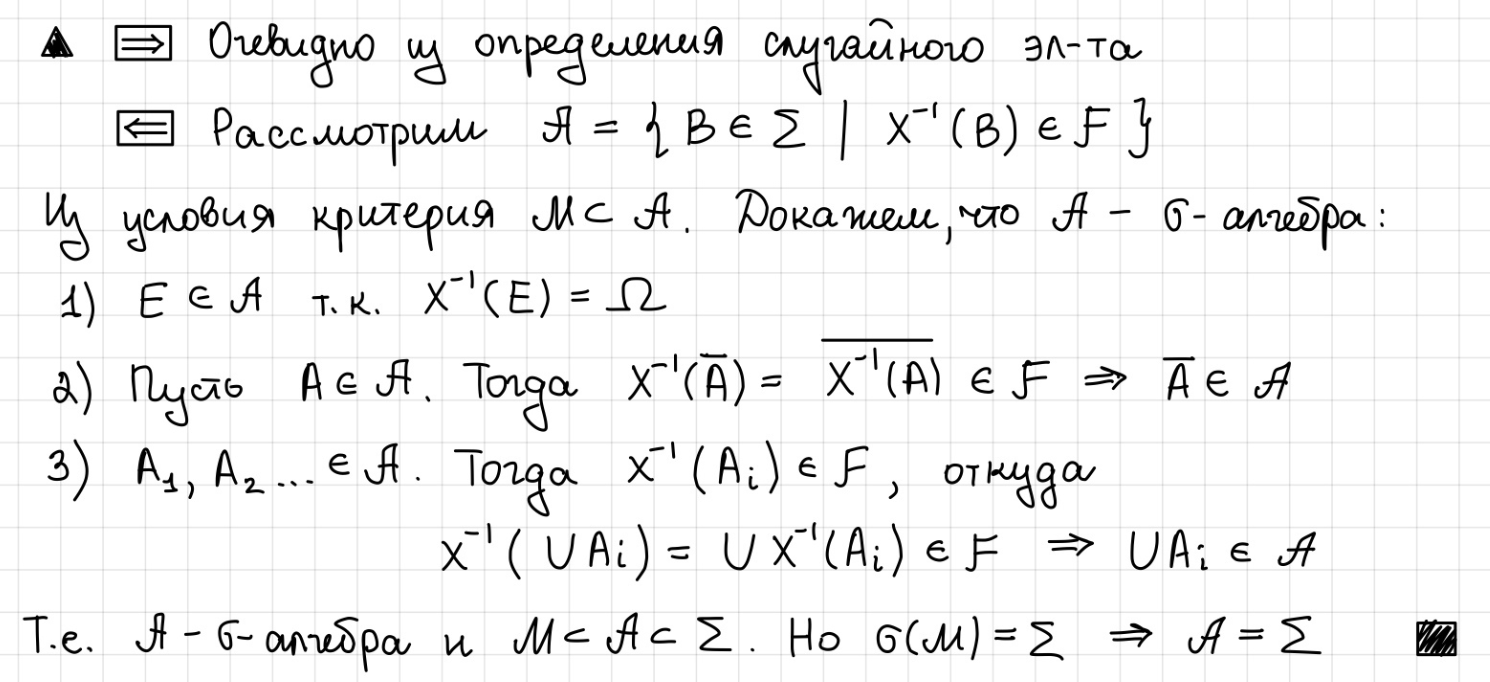
\includegraphics[scale=0.5]{images/izmerimost.png}

\begin{statement}
$\F_X = \{X^{-1}(B), B \in \Sigma\}$ --- $\sigma$-алгебра (порождённая $X$)
\end{statement}
\begin{proof}
\,\newline
\begin{enumerate}
    \item $X^{-1}(E) = \Omega \in \F_X$
    
    \item Если $A \in \F_X$, то $\exists B \in \Sigma$, что $X^{-1}(B) = A$
    
    $\overline{B} \in \Sigma \Rightarrow X^{-1}(\overline{B}) \in \F_X$. Но $X^{-1}(\overline{B}) = \overline{X^{-1}(B)} = \overline{A}$
    
    \item Если $A_1, A_2, \ldots \in \F_X$, то $\exists B_1, B_2, \ldots \in \Sigma: X^{-1}(B_i) = A_i$
    
    $\cup A_i = X^{-1}(\cup B_i) \in \F_X$ (т.к. $\cup B_i \in \Sigma$)
\end{enumerate}
\end{proof}

\textbf{Действия над случайными величинами}

\begin{definition}
$f: \R^n \to \R^k$ --- \textit{борелевская}, если $\forall B \in B(\R^k) : f^{-1}(B) \in B(\R^n)$
\end{definition}

\begin{theorem}
Пусть $\xi$ --- $n$-мерный случайный вектор, $\eta : \Omega \to \R^k$

Тогда $\eta $ --- $\F_{\xi}$-измеримый случайный вектор (то есть $\forall B \in B(\R^k) \eta^{-1}(B) \in F_{\xi}$) $\Leftrightarrow \exists$ борелевская функция $f : \R^n \to \R^k : \eta = f(\xi)$
\end{theorem}

Справа налево очевидно, слева направо оставил б/д.

\begin{statement}
$\xi = (\xi_1, \ldots, \xi_n)$ --- случайный вектор $\Leftrightarrow \xi_1, \ldots, \xi_n$ --- случайные величины.
\end{statement}

\begin{proof}
\:\newline
\begin{itemize}
    \item $i \in \{1, \ldots, n\}, B \in B(\R)$
    
    $\xi_i^{-1}(B) = \{w : \xi_i(w) \in B\} = \{w : \xi(w) \in \R^{i-1} \times B \times \R^{n-i}\} \in \F$
    
    Значит, $\xi_i$ -- случайная величина
    
    \item $\sigma(\{B_1 \times \ldots \times B_n\})=\B(\R^n)$
    
    $\xi^{-1}(B_1 \times \ldots \times B_n) = \{w : \xi(w) \in B_1 \times \ldots \times B_n\} = \{w : \xi_1(w) \in B_1, \ldots, \xi_n(w) \in B_n\} = \bigcap\limits_{i=1}^n \{w : \xi_i(w) \in B_i\} = \bigcap\limits_{i=1}^n \xi_i^{-1}(B_i) \in \F$
\end{itemize}
\end{proof}

\begin{statement}
Любая непрерывная (кусочно-непрерывная) функция является борелевской.
\end{statement}

\begin{corollary}
Если $\xi,\, \eta$ --- случайные величины, то $\xi + \eta,\, \xi - \eta,\, \xi \cdot \eta,\, \frac{\xi}{\eta} \cdot I(\eta \neq 0)$ --- случайные величины
\end{corollary}

\begin{statement}
Если $\xi_1,\, \xi_2,\, \ldots$ --- случайные величины, то $\inf\limits_{n} \xi_n,\: \sup\limits_{n} \xi_n,\: \underset{n \to \infty}{\underline{\text{lim}}} \xi_n,\: \underset{n \to \infty}{\overline{\text{lim}}} \xi_n$ --- случайные величины.
\end{statement}

\begin{proof}
\:\newline
\begin{enumerate}
    \item $\xi = \sup\limits_{n} \ \xi_n$
    
    $\xi^{-1}((-\infty, x]) = \{w: \xi(w) \leqslant x\} = \{w : \forall n \xi_n \leqslant x\} = \bigcap\limits_{n} \xi_n^{-1}((-\infty, x]) \in \F$
    
    \item $\xi = \inf\limits_{n} \ \xi_n$
    
    $\xi^{-1}([x, +\infty)) = \bigcap\limits_{n} \xi_n^{-1}([x, +\infty)) \in \F$
    
    \item $\xi = \underset{n \to \infty}{\overline{\text{lim}}} \xi_n$
    
    $\xi^{-1}((x, +\infty)) = \bigcup\limits_{\varepsilon > 0} \{w\!\!\! : \forall k \exists n \geqslant k \ \xi_n > x + \varepsilon\} = \bigcup\limits_{m \in N} \{w\!\!\! : \forall k \exists n \geqslant k \ \xi_n > x + \frac{1}{m}\} =$
    $= \bigcup\limits_{m}\bigcap\limits_{k}\bigcup\limits_{n \geqslant k} \left\{\xi_n > x + \frac{1}{m}\right\} \in \F$
    
    \item $\xi = \underset{n \to \infty}{\underline{\text{lim}}} \xi_n$
    
    $\xi^{-1}((-\infty, x)) = \bigcup\limits_{\varepsilon > 0} \{w : \forall k \exists n \geqslant k \ \xi_n < x - \varepsilon\} = \bigcup\limits_{m}\bigcap\limits_{k}\bigcup\limits_{n \geqslant k}\left\{\xi_n < x - \frac{1}{m}\right\} \in \F$
\end{enumerate}
\end{proof}